\documentclass[]{article}
\usepackage{float}
\usepackage{graphicx}
\usepackage[svgnames]{xcolor} 
\usepackage{fancyhdr}
\usepackage{fancyvrb}
\usepackage{forest}
\usepackage{tocloft}
\usepackage[hidelinks]{hyperref}
\usepackage{enumitem}
\usepackage[many]{tcolorbox}
\usepackage{listings }
\usepackage[a4paper, total={6in, 8in} , top = 2cm,bottom = 4cm]{geometry}
%\usepackage[a4paper, total={6in, 8in}]{geometry}
\usepackage{afterpage}
\usepackage{amssymb}
\usepackage{pdflscape}
\usepackage{textcomp}
\usepackage{xecolor}
\usepackage{rotating}
\usepackage[Kashida]{xepersian}
\usepackage[T1]{fontenc}
\usepackage{tikz}
\usepackage[utf8]{inputenc}
\usepackage{PTSerif} 
\usepackage{seqsplit}
\usepackage{changepage}


\usepackage{listings}
\usepackage{xcolor}
\usepackage{sectsty}

\setcounter{secnumdepth}{0}
 
\definecolor{codegreen}{rgb}{0,0.6,0}
\definecolor{codegray}{rgb}{0.5,0.5,0.5}
\definecolor{codepurple}{rgb}{0.58,0,0.82}
\definecolor{backcolour}{rgb}{0.95,0.95,0.92}
\definecolor{blanchedalmond}{rgb}{1.0, 0.92, 0.8}
\definecolor{brilliantlavender}{rgb}{0.96, 0.73, 1.0}
 
\NewDocumentCommand{\codeword}{v}{
\texttt{\textcolor{blue}{#1}}
}
\lstset{language=java,keywordstyle={\bfseries \color{blue}}}

\lstdefinestyle{mystyle}{
    backgroundcolor=\color{backcolour},   
    commentstyle=\color{codegreen},
    keywordstyle=\color{magenta},
    numberstyle=\tiny\color{codegray},
    stringstyle=\color{codepurple},
    basicstyle=\ttfamily\normalsize,
    breakatwhitespace=false,         
    breaklines=true,                 
    captionpos=b,                    
    keepspaces=true,                 
    numbers=left,                    
    numbersep=5pt,                  
    showspaces=false,                
    showstringspaces=false,
    showtabs=false,                  
    tabsize=2
}

\lstset{style=mystyle}

 \settextfont[BoldFont={XB Zar bold.ttf}]{XB Zar.ttf}


\setlatintextfont[Scale=1.0,
 BoldFont={LiberationSerif-Bold.ttf}, 
 ItalicFont={LiberationSerif-Italic.ttf}]{LiberationSerif-Regular.ttf}





\newcommand{\inputsample}[1]{
    ~\\
    \textbf{ورودی نمونه}
    ~\\
    \begin{tcolorbox}[breakable,boxrule=0pt]
        \begin{latin}
            \large{
                #1
            }
        \end{latin}
    \end{tcolorbox}
}

\newcommand{\outputsample}[1]{
    ~\\
    \textbf{خروجی نمونه}

    \begin{tcolorbox}[breakable,boxrule=0pt]
        \begin{latin}
            \large{
                #1
            }
        \end{latin}
    \end{tcolorbox}
}

\newtcolorbox{mybox}[2][]{colback=red!5!white,
colframe=red!75!black,fonttitle=\bfseries,
colbacktitle=red!85!black,enhanced,
attach boxed title to top center={yshift=-2mm},
title=#2,#1}

\newenvironment{changemargin}[2]{%
\begin{list}{}{%
\setlength{\topsep}{0pt}%
\setlength{\leftmargin}{#1}%
\setlength{\rightmargin}{#2}%
\setlength{\listparindent}{\parindent}%
\setlength{\itemindent}{\parindent}%
\setlength{\parsep}{\parskip}%
}%
\item[]}{\end{list}}


\definecolor{foldercolor}{RGB}{124,166,198}
\definecolor{sectionColor}{HTML}{ff5e0e}
\definecolor{subsectionColor}{HTML}{008575}

\definecolor{listColor}{HTML}{00d3b9}

\definecolor{umlrelcolor}{HTML}{3c78d8}

\definecolor{subsubsectionColor}{HTML}{3c78d8}

\defpersianfont\authorFont[Scale=0.9]{XB Zar bold.ttf}

\defpersianfont\titr[Scale=1.5]{Lalezar-Regular.ttf}

\defpersianfont\fehrest[Scale=1.2]{Lalezar-Regular.ttf}

\defpersianfont\fehrestTitle[Scale=3.0]{Lalezar-Regular.ttf}

\defpersianfont\fehrestContent[Scale=1.2]{XB Zar bold.ttf}


\sectionfont{\color{sectionColor}}  % sets colour of sections
\subsectionfont{\color{subsectionColor}}  % sets colour of sections
\subsubsectionfont{\color{subsubsectionColor}}


\renewcommand{\labelitemii}{$\circ$}


\renewcommand{\baselinestretch}{1.1}


\renewcommand{\contentsname}{فهرست}

\renewcommand{\cfttoctitlefont}{\fehrestTitle}


\renewcommand\cftsecfont{\color{sectionColor}\fehrestContent\selectfont}
\renewcommand\cftsubsecfont{\color{subsectionColor}\fehrestContent\selectfont}
\renewcommand\cftsubsubsecfont{\color{subsubsectionColor}\fehrestContent\selectfont}
%\renewcommand{\cftsecpagefont}{\color{sectionColor}}

\setlength{\parskip}{1.2pt}

\begin{document}


%%% title pages
\begin{titlepage}
\begin{center}

\textbf{ \Huge{به نام خدا} }
        
\vspace{0.2cm}


\includegraphics[width=0.4\textwidth]{sharif1.png}\\
\vspace{0.2cm}
\textbf{ \Huge{\emph درس برنامه‌سازی پیشرفته} }\\
\vspace{0.25cm}
\textbf{ \Large{ فاز دوم پروژه} }
\vspace{0.2cm}
       
 
      \large \textbf{دانشکده مهندسی کامپیوتر}\\\vspace{0.1cm}
    \large   دانشگاه صنعتی شریف\\\vspace{0.2cm}
       \large   ﻧﯿﻢ سال دوم 01-00 \\\vspace{0.10cm}
      \noindent\rule[1ex]{\linewidth}{1pt}
استاد:\\
    \textbf{{دکتر محمدامین فضلی}}



    \vspace{0.20cm}

   مهلت ارسال:\\
    \textbf{{چک پوینت 8 خرداد}}\\
    \textbf{{چک پوینت 15 خرداد}}\\
    \textbf{{فاز دوم: 22 خرداد}}\\
    \textbf{{ساعت 23:59:59}}

    \vspace{0.10cm}
مسئول پروژه:\\
    \textbf{\authorFont{امیرمهدی کوششی}}
    
        \vspace{0.10cm}
مسئول فاز دوم:\\
    \textbf{\authorFont{سیاوش رحیمی شاطرانلو}}
    
        \vspace{0.10cm}
طراحان فاز دوم:\\
    \textbf{\authorFont{علی پاشا منتصری، امیرحسین رازلیقی، عرفان مجیبی، هومان کشوری، محمد خسروی، سوگند صالحی، بنیامین ملکی، عرفان صدرائیه، کامیار کازری، علی ثالثی، امیرمحمد فخیمی، علی نظری، امیرحیسن رازلیقی}}
    
        \vspace{0.05cm}
مسئولین تنظیم مستند:\\
    \textbf{\authorFont{امیرمهدی کوششی}}
    

\end{center}
\end{titlepage}
%%% title pages


%%% header of pages
\newpage
\pagestyle{fancy}
\fancyhf{}
\fancyfoot{}
\cfoot{\thepage}
\lhead{فاز دوم}
\rhead{
\includegraphics[width=0.1\textwidth]{sharif.png}\\
دانشکده مهندسی کامپیوتر
}
\chead{پروژه برنامه‌سازی پیشرفته}
%%% header of pages
\renewcommand{\headrulewidth}{2pt}

\KashidaOff



\tableofcontents

\newpage

 \Large \textbf{\\\\
}


\section*{{\titr نکات قابل توجه}}
\addcontentsline{toc}{section}{{\fehrestContent نکات قابل توجه}}
\begin{itemize}
\item
پس از اتمام این فاز، در گیت خود یک تگ با ورژن \lr{"v2.0.0"} بزنید. در روز تحویل حضوری این tag بررسی خواهد شد و کدهای پس از آن نمره‌ای نخواهد گرفت. برای اطلاعات بیش‌تر در مورد شیوه ورژن‌گذاری، می‌توانید به
 \href{https://semver.org/}{\textcolor{blue}{\underline{این لینک}}}
 مراجعه کنید. البته برای این پروژه صرفا رعایت کردن همان ورژن گفته شده کافیست، اما خوب‌ است که با منطق ورژن‌بندی هم آشنا بشوید.

\item
در روز تحویل حضوری مشارکت تمام اعضای تیم در پروژه بررسی خواهد‌ شد و در صورت عدم مشارکت بعضی از اعضا، نمره‌ی ایشان برای آن فاز پروژه "صفر" لحاظ می‌گردد. مشارکت، با توجه به commit های افراد تیم در مخزن گیت‌هاب پروژه بررسی می‌شود.

\item
در هر فاز می‌توانید سه روز تاخیر به ازای کسر نمره داشته‌ باشید که به ازای هر روز آن، ۱۰ درصد از نمرهٔ آن فاز را از دست خواهید‌ داد. در مجموع سه‌فاز پروژه، سه روز تاخیر نیز بخشیده خواهد‌ شد.

\item
به ازای هر ساعتی که پروژه را زودتر تحویل دهید، ۱۵ دقیقه به مهلت تاخیر بدون کسر نمره شما اضافه خواهد‌ شد. این مقدار حداکثر یک روز خواهد‌ بود که در صورت ارسال ۴ روز زودتر از ددلاین به شما تعلق خواهد گرفت. \textbf{بنابراین ددلاین‌های پروژه تحت هیچ شرایطی تمدید نخواهد‌ شد.} توصیه می‌شود با برنامه‌ریزی مناسب به ددلاین‌های درس پایبند باشید.

\item
در صورت کشف تقلب از هریک از تیم‌ها، برای بار اول منفی نمرهٔ آن فاز برای آن تیم ثبت می‌شود و برای بار دوم، نمرهٔ منفی کل پروژه برای تیم لحاظ خواهد‌ شد که معادل مردود شدن در درس است.

\end{itemize}

\newpage

\section*{{\titr مقدمه}}
\addcontentsline{toc}{section}{{\fehrestContent مقدمه}}

\subsection*{{\titr نکات}}

\addcontentsline{toc}{subsection}{{\fehrestContent نکات}}

\begin{itemize}

 \item در طراحی بازی یکی از نکاتی که باید در نظر داشت \lr{user friendly} بودن محیط بازی است به این معنی که در استفاده از آن ابهامی وجود نداشته باشد و به سادگی بتوان فهمید که هر عنصر بیانگر چه چیزی است یکی از را‌ه‌های رسیدن به آن حذف هرگونه عنصر اضافی و همچنین استفاده از \lr{sprite} های مناسب برای هر قسمت است.
 
 \item استفاده از فونت و رنگ مناسب در محیط بازی اهمیت دارد به این صورت که نوشته‌ها باید کاملا واضح و خوانا باشند. برای مثال استفاده از رنگ متنی که تفاوت زیادی با رنگ \lr{background} ندارد خوانایی متن را کاهش می‌دهد.
\item در هر بخش بعضا یک چینش برای آن بخش پیشنهاد داده شده است اما هیچ اجباری برای طراحی صفحه به آن صورت نیست و می‌توانید خواسته‌های هر بخش را هر طور که مایلید پیاده‌سازی کنید اما دقت کنید که تمام قابلیت‌های خواسته شده باید در پیا‌ده‌سازی شما وجود داشته باشد.
\end{itemize}

\subsection*{{\titr کلیات پروژه}}
\addcontentsline{toc}{subsection}{{\fehrestContent کلیات پروژه}}

در این فاز، قرار است برای منطقی که در فاز 1 پروژه پیاده سازی کردید، یک گرافیک بالا بیاورید. نحوهٔ ارتباط با کاربر نیز از طریق همین گرافیک خواهد بود. توجه داشته باشید که در فاز سوم پروژه، باید سیستم را طبق یک معماری سرور-کلاینت طراحی کنید. در معماری اکثر بازی‌هایی که به این شکل انجام می‌شوند، منطق بازی در سرور و مستقل از واسط کاربری سمت کلاینت و کاربر است. هر چند برای فاز دوم نیاز به این مسئله ندارید ولی خوب‌ است که از الآن طراحی خوبی داشته باشید.
\\
همچنین مواردی که در داک توضیحات بازی آمده بود اما در فاز 1 پیاده سازی نکرده بودید را باید در این فاز پیاده سازی کرده و گرافیک مناسب آن قسمت را هم پیاده سازی کنید.
\begin{enumerate}[label={نکته \arabic*:}]
	\item
دقت کنید که دو داک در اختیار شما قرار می گیرد، یک داک توضیحات کاملی از بازی است، و همه چیز راجع به بازی در آن توضیح داده شده است، یک داک دیگر مربوط به فاز دوم پروژه شما می باشد که همین داک است. همچنین در کنار این داک‌ها یک فایل زیپ از asset هایی که ممکن است برای طراحی گرافیک بازی به آن‌ها نیاز پیدا کنید نیز آمده است.
\item
 تمامی اطلاعات، اعم از اطلاعات کاربران و... باید در خارج از برنامه (مثلا روی فایل) ذخیره شوند و پس از \lr{terminate} شدن برنامه و اجرای مجدد آن، بصورت خودکار اطلاعات قبلی خوانده شود و قابل دسترسی باشد. برای این کار می‌توانید از ابزارهای کار با \lr{Json} در جاوا، مثل
  \href{https://www.tutorialspoint.com/gson/gson_quick_guide.htm}{\textcolor{blue}{\lr{Gson}}}
یا
  \href{https://github.com/amogilev/yagson}{\textcolor{blue}{\lr{YaGson}}}
   استفاده‌ کنید.

\end{enumerate}

\newpage


\section*{{\titr چک پوینت اول}}
\addcontentsline{toc}{section}{{\fehrestContent چک پوینت اول}}
\section*{{\titr جزئیات}}
\addcontentsline{toc}{section}{{\fehrestContent جزئیات}}

\subsection*{{\titr منوها}}
\addcontentsline{toc}{subsection}{{\fehrestContent منوها}}

\begin{itemize}
\item تمامی منوهای پیاده سازی شده باید از منوی اصلی در دسترس باشند و همچنین امکان برگشت از آن‌ها به منوی اصلی نیز باید وجود داشته باشد.

\item تمامی منوها باید دارای background مناسب باشند.
\item  اگر در حین انجام هر عملیاتی به خطا برخوردید باید این خطا به طور مناسب نشان داده شود. خطا را با توجه به نوع آن می‌توانید در متنی زیر دکمه ی انجام عملیات، زیر element ورودی کاربر و یا در قالب یک up pop را نشان دهید.
\item \textbf{امتیازی:} تغییر شکل نشان گر موس در بازی نمره امتیازی دارد. مثلا در هنگام حمله شکل آن به صورت دیگری در بیاید و یا در صورتی که روی گزینه غیرفعالی قرار گرفت به شکل ضربدر در بیاید. پیاده سازی این مورد برای یک مورد برای گرفتن نمره امتیازی آن کافی است. 
\end{itemize}



\subsubsection*{{\titr منوی ثبت‌نام و ورود}}
\addcontentsline{toc}{subsection}{{\fehrestContent منوی ثبت‌نام و ورود}}
\begin{itemize}
    \item \textbf{ثبت‌نام(Register):} سه ورودی نام کاربری، نام مستعار و رمز از کاربر گرفته شده و در صورت عدم وجود خطا حساب کاربری ساخته می‌شود و پیام موفقیت نیز نمایش داده می‌شود. در صورت وجود خطا نیز باید خطای مرتبط به کاربر نشان داده‌ شود. نمایش خطاها یا پیغام موفقیت باید در قالب یک pop-up یا یک پیغام در زیر دکمه ثبت نام باشد.
 \item \textbf{عکس پروفایل:} هر کاربر باید یک عکس پروفایل نیز داشته باشد. با ساخت حساب کاربری لازم است یک عکس به صورت پیش فرض یا رندوم برای کاربر تنظیم شود که در آینده بتواند آن را تغییر دهد.
\item \textbf{ورود(Login):} با دریافت نام کاربری و رمز عبور از کاربر در صورت معتبر بودن، باید کاربر لاگین شده و وارد منوی اصلی شود. اگر نام کاربری و رمز عبور مطابقت نداشتند، باید خطای مناسب نمایش داده شود.
\end{itemize}



\subsubsection*{{\titr منوی اصلی}}
\addcontentsline{toc}{subsection}{{\fehrestContent منوی اصلی}}
\begin{itemize}
\item باید امکان Logout کردن از حساب در این منو وجود داشته باشد به طوری که پس از Logout به منوی ثبت‌نام/ورود منتقل شویم.

\item تمامی منوهای پیاده سازی شده باید از منوی اصلی در دسترس باشند و همچنین امکان برگشت از آن‌ها به منوی اصلی نیز باید وجود داشته باشد.
\end{itemize}



\subsubsection*{{\titr منوی پروفایل}}
\addcontentsline{toc}{subsection}{{\fehrestContent منوی پروفایل}}
\begin{itemize}
\item \textbf{عکس پروفایل:} همانطور که در منوی ثبت‌نام اشاره شد، هر کاربر یک عکس پروفایل دارد که در هنگام ثبت‌نام به یک تصویر پیشفرض قرار می‌گیرد. کاربر باید بتواند در منوی پروفایل عکس پروفایل خود را تغییر دهد، به این صورت که شما چند عکس پیشفرض(حداقل 4تا) به اون نمایش دهید و یکی را انتخاب کند. همچنین امکان انتخاب عکس پروفایل از میان فایل‌های موجود روی کامپیوتر نیز باید وجود داشته باشد.

\item \textbf{تغییر رمزعبور password change} باید قابلیت تغییر رمز عبور وجود داشته باشد، به این صورت که با وارد کردن پسورد کنونی و پسورد جدید، کاربر بتواند پسورد خود را تغییر دهد. در صورت وجود هرگونه خطا، باید آن را در قالب مناسب نمایش دهید.

\item \textbf{تغییر نام مستعار nickname change} باید قابلیت تغییر نام مستعار وجود داشته باشد. در صورت وجود هرگونه خطا(به طور مثال وجود کاربری دیگر با این نام مستعار)، باید آن را در قالب مناسب نمایش دهید.

\end{itemize}

\subsubsection*{{\titr منوی بازی}}
\addcontentsline{toc}{subsection}{{\fehrestContent منوی بازی}}

  در این بخش باید منوی مربوط بازی را پیاده‌سازی کنید. بخشی از منطق این منو را در فاز اول کامل کرده‌اید و بخشی دیگر را نیاز است که در این فاز تکمیل کنید. در این بخش نیازمندی‌های این منو شرح داده شود.

\begin{itemize}
\item اولین و اصلی ترین نیاز این بخش، قابلیت شروع بازی است که در فاز یک هم پیاده‌سازی شده است و در این فاز یک رابط گرافیکی برای استفاده از آن باید قرار دهید.

\item همانطور که می‌دانید، در فاز سوم شما باید پروژه را بر بستر شبکه قرار دهید و به این ترتیب می‌توان از دو سیستم متفاوت، به بازی و نبرد با یکدیگر بپردازید. قابلیتی که در این فاز در این منو باید قرار دهید، این است که بتوان بر اساس نام کاربری شخصی، برای او دعوتنامه به مبارزه بفرستید و بتوانید با شخص خاصی که مدنظر خودتان است، به بازی بپردازید. کاربرد این بخش در منو، در فاز سوم مشخص می‌شود و در این فاز صرفا قالب آن را باید ایجاد کنید.

\item همانطور که می‌دانید در این بازی می‌توان با تعداد بیش از ۲ نفر هم به بازی پرداخت. در نتیجه باید بخشی برای تعیین تعداد افرادی که می‌خواهیم با آن‌ها بازی کنیم، قرار دهید تا در فاز ۳ که موتور جستجو پیدا کردن حریف را پیاده‌سازی می‌کنید، بتوانید تعیین کنید تمایل دارید با چند نفر به بازی بپردازید.

\item دقت کنید که نقشه‌های موجود در بازی متنوع است و بر اساس تعداد افراد می‌تواند وسعت متفاوتی هم داشته باشد. در نتیجه باید نقشه بازی را بر اساس تعداد افراد موجود در آن نبرد مشخص کنید و قابلیت جداگانه‌ای برای انتخاب ابعاد نقشه هم داشته باشید.

\item همانطور که می‌دانید بازی online یا multiplayer قابلیت stop یا save و load ندارد ولی در این فاز چون هنوز بازی چند نفره هم در یک سیستم انجام می‌شود، باید قابلیت save کردن بازی و سپس load آن را داشته باشید. به طوری که با terminate شدن برنامه و سپس راه‌اندازی مجدد، load ها قابل دسترسی باشند.
در واقع شما باید یک قسمتی را در منوی بازی درنظر بگیرید که درصورتی یک بازی‌ای از قبل stop شده بود(در واقع کسی هنوز نبرده است) رابتواند استارت کند و از همان استیتی که stop شده بود، به بازی ادامه دهد.
\item در مورد بحث save و load بازی یک قابلیت که باید آن را در نظر بگیرید، این است که بتوان save auto را فعال کرد. برای این منظور، کاربر باید از بین چند گزینه، بتواند دوره‌های save auto را انتخاب کند. به عنوان مثال، بعد از هر round یا بعد از اشغال شدن یک شهر یا موارد دیگر که بسته به سلیقه خود می‌توانید آن‌ها را قرار دهید.

\item همچنین چون فایل‌های save را باید روی hard disk قرار دهید، ممکن است در طول بازی تعداد بسیار زیادی از این فایل‌ها تولید شود که می‌توانند مشکل‌زا باشند. پس در این منو باید بتوان مشخص کرد که چه تعداد از فایل save ها باقی بماند. به عنوان مثال اگر عد ۵ برای این مورد انتخاب شد، در طول بازی که auto save ها را انجام می‌دهید، وقتی فایل ششم در حال نوشته شدن بود، فایل اول باید از روی disk باید پاک شود. البته دقت کنید که این مورد فقط برای فایل‌های تولید شده از بحث save auto است و save هایی که کاربر آن‌ها را ایجاد می‌کند، کاملا مجزا باید باشد و به طور کامل باید نگهداری شوند.

\item همانطور که متوجه شدید، موارد این منو مقداری زیاد است و کاربر شاید دقیق متوجه نشود هر گزینه برای چه کاری است پس باید این قابلیت را هم پیاده‌سازی کنید که با نگه داشتن موس روی هر مورد، یک tooltip برای آن گزینه باز شود و شرح دهد که این مورد چه کاری انجام می‌دهد. منظور از نگه داشتن موس روی آن، کلیک کردن و نگه داشتن موس در حالت کلیک شده نیست و منظور همان hover کردن روی گزینه ها است.

\item \textbf{امتیازی} در حالت عادی، افراد به طور رندوم روی نقشه قرار می‌گیرند ولی باید قابلیتی موجود باشد که بتوان مکان اولیه هر بازیکن روی نقشه را مشخص کرد. برای این کار باید با زدن ctrl + shift + c به ترتیب پنلی باید باز شود تا در آن بتوان کد تقلب را وارد کرد و با وارد کردن کد تقلب که می‌تواند هر چیزی باشد، کاربر می‌تواند مکان اولیه خود روی نقشه را مشخص کند و دیگر رندوم نیست این موضوع.

\item \textbf{امتیازی} در بازی اصلی هم مشاهده کردید که حرکت سربازها و حمله‌ها و … زمانبر است و می‌توان سرعت بازی را هم مشخص کرد. این قابلیت در پروژه شما هم باید باشد که بتوان سرعت بازی را از بین چند گزینه موجود، انتخاب کرد و بازی با همان سرعت جریان یابد.

\end{itemize}



\subsubsection*{{\titr منوی امتیازات}}
\addcontentsline{toc}{subsection}{{\fehrestContent منوی امتیازات}}

در این منو ، همانطور که از نامش مشخص است ، باید جدول امتیازاتی برای بازیکنان بازی در نظر بگیرید . طراحی ظاهری این جدول بنابر سلیقه و طراحی خودتان است اما در این طراحی ، موارد زیر را در نظر بگیرید :
۱- بازیکنان باید بر اساس این ترتیب sort شوند : امتیاز آنها - زمانی که به آن امتیاز رسیده اند - ترتیب الفبایی نام آنها \\
برای مثال ، در بین ۱۰ بازیکن بازی ، در ابتدا نام آنهایی می آید که بیشترین امتیاز را از بازی کسب کرده اند (بیشترین برد ) . اگر دو بازیکن ، امتیاز یکسانی داشته باشند ، باید به “زمان رسیدن به آن امتیاز“ دقت کنیم . مثلا بازیکن X و Y هر دو ۴ برد داشته اند اما بازیکن X ، آخرین بردش در ساعت 17:00 بوده و بازیکن Y آخرین بردش در ساعت 14:00 بوده . پس در جدول امتیازات ، نام y بالاتر از نام x باید قرار بگیرد . در نهایت اگر برای دو بازیکن ، هر دو این پارامتر ها ( امتیاز و زمان ) یکسان بود ، باید آنها را بر اساس حروف الفبای انگلیسی (lexicographically) مرتب کنید .\\
توجه کنید که باید در جدول ، برای هر کاربر ، نام آن کاربر ، آواتار او ، امتیاز او و زمان آخرین بردش را نمایش بدهید . هم چنین باید برای هر کاربر ، آخرین زمانی که او آنلاین بوده ( در بازی لاگین بوده ) را نمایش بدهید .
۲- باید ردیف user ی که هم اکنون در بازی لاگین کرده است و در حال تماشای جدول امتیازات است را با رنگ و style متفاوتی ( به سلیقه ی خودتان ) نسبت به دیگر ردیف های جدول امتیازات نمایش دهید .


\subsubsection*{{\titr منوی چت}}
\addcontentsline{toc}{subsection}{{\fehrestContent منوی چت}}

در این منو ، شما باید یک chatroom برای بازی خود طراحی کنید . توجه کنید که این چت روم ، بصورت یک منوی جداگانه است و داخل بازی نیست. طراحی ظاهری و style های این منو به عهده ی خودتان است و میتوانید با سلیقه ی خودتان آن را طراحی کنید . مهم است که چت روم شما این ویژگی ها را داشته باشد : \\
۱- چت روم شما باید ۳ بخش مختلف داشته باشد : public chat - private chats - rooms\\
۲- در بخش public chat ، تمام بازیکنان میتوانند بدون محدودیت با همدیگر صحبت کنند و پیام بفرستند .\\
۳- در بخش private chats ، هر بازیکن میتواند بازیکن دیگری را بر حسب نام او در بازی ، search کند و با او وارد یک چت خصوصی شود .\\
۴- در بخش rooms ، هر بازیکن میتواند تعدادی room با نام های مختلف ایجاد کند و در هر room ، بازیکنان دیگری را که میخواهد ( با search کردن نام آنها ) به آن room اضافه کند و با آنها چت کند ( مشابه group chat در اپلیکیشن های معروف ! )\\
۵- در هر بخش ، کاربر باید توانایی edit کردن پیام های خود ، پاک کردن پیام های خود ( برای خودش ) و پاک کردن پیام های خود (برای خودش و دیگران) را داشته باشد\\
۶- هر پیام باید حاوی این اطلاعات باشد : نام فرستنده - زمان ارسال - متن پیام - آواتار شخص فرستنده - علامتی برای نمایش اینکه پیام ارسال شده است - علامتی برای اینکه پیام seen شده است ( مشابه اپلیکیشین های چت معروف ) \\
۷- دقت کنید که تمام اطلاعات (history) مربوط به چت های مختلف ، باید پس از بستن بازی و باز کردن دوباره ی آن ، حفظ شود . برای این کار میتوانید از ذخیره سازی اطلاعات مربوطه در فایل و خواندن مجدد اطلاعات از فایل ، استفاده کنید .
توجه کنید که در نحوه ی طراحی و پیاده سازی این منو ، دستتان باز است و آزادی کامل دارید . نکته ی مهم این است که موارد ذکر شده در بالا را حتما رعایت کنید.\\
دقت کنید که قابلیت پیام دادن در فاز بعدی چک می‌شود، و در این فاز فقط مهم است شما گرافیک مد نظر را برای چت پیاده سازی کنید و نیازی به پیام دادن هر کاربر نمیباشد.

\subsubsection*{{\titr ساخت مپ دستی (امتیازی)}}
\addcontentsline{toc}{subsection}{{\fehrestContent ساخت مپ دستی(امتیازی)}}

بعنوان یک قابلیت امتیازی می‌توانید امکان ساختن نقشه دلخواه برای کاربر را فراهم کنید. 

\begin{itemize}
\item انتظار می‌رود کاربر بتواند نوع زمین در هر کاشی را از بین انواعی که وجود دارد انتخاب کند.

\item انتظار می‌رود قابلیت تعیین نوع مرز وجود داشته باشد. (مثلا ایجاد رودخانه)

\item انتظار می‌رود کاربر بتواند ویژگی‌های ممکن برای هر زمین را تعیین کند؛ مثلا در برخی کاشی‌ها جنگل قرار دهد.(توجه کنید محدودیت‌های هر ویژگی باید رعایت شود؛ مثلا جلگه باید در کنار رود باشد.) 

\item انتظار می‌رود کاربر بتواند منابع مد نظر برای هر کاشی را (با توجه به محدودیت‌ها) مشخص کند.

\item در صورت پیاده‌سازی این قسمت، شما باید نقشه‌های ساخته شده را ذخیره کنید، و همچنین در منوی بازی یک قسمت برای انتخاب نقشه از بین نقشه‌های ساخته شده نیز اضافه کنید تا اگر کاربران خواستند در نقشه‌هایی که خودشان ساخته‌اند به بازی بپردازند.

\end{itemize}









\section*{{\titr چک پوینت دوم}}
\addcontentsline{toc}{section}{{\fehrestContent چک پوینت دوم}}


\section*{{\titr جزئیات}}
\addcontentsline{toc}{section}{{\fehrestContent جزئیات}}


\subsection*{{\titr دیدن نقشه (navigation)}}
\addcontentsline{toc}{subsection}{{\fehrestContent دیدن نقشه (navigation)}}

پیاده‌سازی navigation در نقشه به این صورت است که باید با فشردن هر کدام از کلیدهای بالا، پایین، چپ و راست نقشه جابه‌جا شود و یک ردیف جدید از کاشی‌ها نشان داده شود؛ با این کار می‌توانید تا انتهای نقشه بروید ولی نمی‌توانید از نقشه خارج شوید(در نظر داشته باشید می‌توانید به گونه دیگری این قابلیت را پیاده‌سازی کنید ولی در طراحی شما navigation در مپ بازی باید امکان‌پذیر باشد).
نیاز به نَرم ظاهر شدن کاشی‌های نقشه نیست و صرفا ظاهر شدنشان کافیست.


\subsection*{{\titr war of fog}}
\addcontentsline{toc}{subsection}{{\fehrestContent war of fog}}

در نقشه 3 مدال کاشی داریم :

\begin{itemize}
    \item کاشی‌هایی که در حال حاضر معلوم هستند(visible)
\item کاشی‌هایی که کشف شده ولی در این زمان معلوم نیستند(revealed)
\item کاشی‌هایی که کلا کشف نشده و در war of fog قرار دارند(war of (fog
\end{itemize}

 حال باید به این صورت عمل شود که کاشی‌های visible کاملا در دیدرس بوده و هر تغییراتی در آنها به صورت زنده قابل مشاهده است.
بر روی کاشی هایی که قبلا کشف شده‌اند اما اکنون دیدی بر آنها نداریم(حالت دوم) یک سایه تیره قرار دارد ، تغییرات آنها قابل مشاهده نیست و فقط نوع زمین کاشی قابل مشاهده است.
کاشی‌هایی نیز که در war of fog قرار دارند یک لایه ابر سفید بر روی آن‌هاست که در آن‌ها دیدن زمین کاشی نیز مقدور نیست.
در صورت نزدیک شدن نیروها به کاشی‌های war of fog ، آن‌ها به کاشی‌های revealed تبدیل می‌شوند.






\subsection*{{\titr panel info}}
\addcontentsline{toc}{subsection}{{\fehrestContent panel info}}
پنل اینفو بالای صفحه نمایش بازیکن قرار دارد و اطلاعاتی را به ما می‌دهد(مطابق با داک توضیحات بازی)

\begin{itemize}
\item  سمت چپ آن میزان سکه‌ها، شادی و علم نشان داده می‌شود. همچنین باید تکنولوژی در حال کار نشان داده شود.

\item در کنار هر مورد باید آیکون مربوطه نیز قرار داشته باشد.

\item می‌توانید از bar status و Research Current عکس زیر الهام بگیرید.

\item اگر یک یونیت توسط بازیکن انتخاب شده بود باید در قسمتی کوچکی از گوشه صفحه اطلاعات یونیت انتخاب شده نمایش داده شود.

\item دکمه‌های setting برای نمایش تنظیمات بازی و turn next هم برای پایان نوبت باید وجود داشته باشند. 

\end{itemize}

\begin{figure}[H]
    \centerline{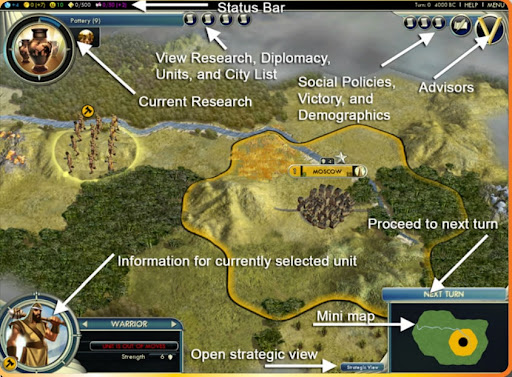
\includegraphics[scale=0.8]{resources/infopanel.jpg}}
\end{figure}



\subsection*{{\titr زمین ویژگی‌ها و منابع Resources) & Features & (Terrain}}
\addcontentsline{toc}{subsection}{{\fehrestContent زمین ویژگی‌ها و منابع Resources) & Features & (Terrain}}

همانطور که در فاز اول پروژه دیدید، این بازی از کاشی‌های شش‌ضلعی تشکیل شده‌ است که زمین بازی را شکل می‌دهند. این کاشی‌ها دارای انواعی بودند. پیاده‌سازی گرافیکی شما باید به گونه‌ای باشد که از رنگ و تصویر این کاشی‌ها تفاوت نوع آن‌ها مشخص باشد (انواعی از زمین که با آن‌ها در فاز قبلی آشنا شدید).
همچنین بسیاری از این کاشی‌ها دارای ویژگی‌های (features) بخصوصی هستند که لازم است شما به نحو مناسبی وجود  این ویژگی ها را در رابط گرافیکی خود نمایش دهید. به طوری که از کاشی‌های بدون آن feature متمایز باشند.
توجه داشته باشید که لازم است، منابع (Resources) و همچنین مقادیر(Values (Terrain مربوط به هر کاشی از زمین بازی را به نحو مناسبی نمایش دهید. به طور مثال می‌توانید اینگونه عمل کنید که هنگامی که یک کاشی از بازی select شد، اطلاعات مربوط به  آن در یک pop-up به کاربر نشان داده شود. همچنین نیاز است که در نمایش این اطلاعات منابع را با استفاده کردن از تصاویر و روش‌های دیگر، به خوبی از یکدیگر متمایز کنید.
در تمامی موارد بالا، لازم است که تاثیراتی که هر کدام از ویژگی‌ها یا منابع بر آن کاشی از زمین بازی گذاشته‌اند را نیز به طرز مناسبی به اطلاع کاربر برسانید.




\subsection*{{\titr خرابه‌ها (Ruins)}}
\addcontentsline{toc}{subsection}{{\fehrestContent خرابه‌ها (Ruins)}}

این نوع خاص از کاشی‌ها در فاز دوم به پروژه شما اضافه می‌شوند(توضیح آن‌ها در داک بازی آمده ولی در فاز 1 ضروری نبود). در این خانه‌های زمین بازی، جایزه‌ها و منافع Benefits) (Ruin پنهانی وجود دارد که تا پیش از کشف شدن آنها، نباید به کاربر نشان داده شود. به محض اینکه یک بازیکن آن‌ها را کشف کرد، این منافع (مثلا از طریق یک (pop-up به اطلاع‌اش برسد. 


\subsection*{{\titr ساختمان‌ها}}
\addcontentsline{toc}{subsection}{{\fehrestContent ساختمان‌ها}}

ساخت ساختمان ها در منوی تولید در صفحه شهر انجام میشود. در داخل منوی تولید فقط ساختمان هایی که در آن لحظه امکان تولید دارند باید نمایش داده شود. همچنین میزان تولید مورد نیاز برای ساخت آن ساختمان باید در منوی تولید نمایش داده شود.


\subsection*{{\titr غذا، طلا، شادی}}
\addcontentsline{toc}{subsection}{{\fehrestContent غذا، طلا، شادی}}

\begin{itemize}
\item مقدار غذا باید در صفحه شهر نمایش داده شود. همچنین جمعیت و تعداد ترن که جمعیت افزایش/کاهش پیدا می‌کند باید قابل نمایش باشد.
\item مقدار طلا باید در نوار وضعیت نمایش داده شود.

\item شادی تمدن شما باید در نوار وضعیت bar) (status صفحه اصلی نمایش داده شود.

\item با نگه داشتن نشانگر موس روی این عدد ، یک تصویر لحظه ای از جمعیت خود نمایش داده شود که happiness و unhappiness چقدر است.
\end{itemize}


\subsection*{{\titr منطق موارد پیاده‌سازی نشده در فاز 1}}
\addcontentsline{toc}{subsection}{{\fehrestContent منطق موارد پیاده‌سازی نشده در فاز 1}}

در فاز اول پروژه، یک سری از موارد بود که پیاده‌سازی نشده بود،(مانند جنگ، برد و باخت و ... (به جز ساختمان و خرابه که در این چک پوینت آمده است و باید هم منطق و هم گرافیک آن پیاده‌سازی شود)) باقی موارد را شما باید در این چک پوینت منطق آن‌ها را پیاده سازی کنید، اما نیازی به پیاده‌سازی گرافیک آن‌ها نیست، و در چک پوینت بعدی باید گرافیک را برای این موارد بالا بیاورید.


\section*{{\titr فاز دوم}}
\addcontentsline{toc}{section}{{\fehrestContent فاز دوم}}


\section*{{\titr جزئیات}}
\addcontentsline{toc}{section}{{\fehrestContent جزئیات}}


\subsection*{{\titr یگان‌ها}}
\addcontentsline{toc}{subsection}{{\fehrestContent یگان‌ها}}

\begin{itemize}
\item هر یگان باید با شکل مناسبی در نقشه نشان داده شود.

\item اطلاعات و ویژگی‌های مربوط به هر یگان باید روی یگان‌ها قابل مشاهده باشد (مانند MP و (CS. برای پیاده‌سازی این قسمت اطلاعات مخصوص یگان می‌تواند پس از انتخاب آن یگان به کاربر نمایش داده شود.

\item برای جابه‌جایی یگان‌ها کافیست که یگان از مبدا به مقصد منتقل شود(نیازی به پیاده‌سازی انیمیشن جابه‌جا شدن یگان‌ها نیست).

\item باید راهی برای انجام عملیات‌های مربوط به یگان‌ها پیاده سازی کنید. مثلا برای خوابیدن، باید گزینه‌ای برای خواباندن یگان‌ها داشته باشید. به همین صورت، باید حالت آماده‌باش، تقویت، تقویت تا ترمیم کامل، مستقر شدن، آماده‌سازی حمله از راه دور، حمله از راه دور، غارت، پیدایش شهر، لغو، بیدار شدن و حذف را پیاده سازی کنید. توجه کنید که پس از انجام هر یک از این عملیات‌ها، باید تغییر مشهودی در یگان‌ها صورت بگیرد (شکل و ظاهر یگان‌ها تغییر کند).

\item اگر در مسیر جابه‌جایی، یگان‌ها به جایی برخورد کنند که توانایی عبور از آن را نداشته باشند باید قبل از شروع دستور حرکت از بازیکن پرسیده شود که آیا می‌خواهد یگان‌هایش تا قبل از محل غیر قابل عبور جابه‌جا شوند یا خیر.

\item در صورت حمله یگان حریف به یگان خودی یا بالعکس نتیجه حمله باید به کاربر اطلاع داده شود(به صورت pop-up یا مشابه آن).  

\end{itemize}

\subsection*{{\titr شهرها}}
\addcontentsline{toc}{subsection}{{\fehrestContent شهرها}}

\begin{itemize}
\item بنر شهر: بنر شهر باید در نقشه قابل دیدن باشد و جمعیت آن شهر معلوم باشد. علاوه بر موارد گفته شده در داک، با کلیک روی بنر شهر باید وارد صفحه شهر شویم. با ورود به صفحه شهر باید تابلوی خروجی شهر(این که چقدر آن شهر غذا، طلا، … تولید می‌کند) را ببینیم. در این تابلوها برای هر کدام از منابع گفته شده باید یک لوگو هم نمایش داده شود.

\item درون صفحه شهر یک دکمه برای خرید تایل و یک دکمه برای بازگشت به مپ اصلی باید تعبیه شود. در صفحه شهر باید مکانیزمی برای قفل کردن یک شهروند به یک کاشی و حذف شهروند از یک کار هم تعبیه شود.

\item در صفحه شهر باید پنلی برای شهروندان بیکار نیز نمایش داده شود. توضیحات مربوط به این منو در داک بازی آمده است. البته نیازی نیست در صورت نبودن شهروند بیکار منو را پنهان کنید.

\item مطابق داک بازی باید پنل تولید در صفحه شهر نمایش داده شود. همچنین باید بتوان از طریق این پنل ساختمان و یونیت در حال ساخت توسط شهر را مشاهده و یا تغییر داد.

\item باید در صفحه شهر یک دکمه purchase موجود باشد که با کلیک روی آن منوی خرید باز شود و باید امکان خرید ساختمان یا یونیت مورد نظر وجود داشته باشد.

\end{itemize}

\begin{figure}[H]
    \centerline{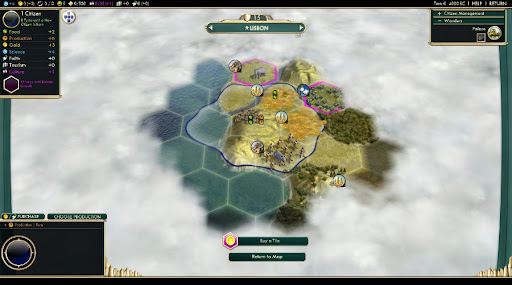
\includegraphics[scale=0.8]{resources/cities.jpg}}
\end{figure}

\subsection*{{\titr تکنولوژی}}
\addcontentsline{toc}{subsection}{{\fehrestContent تکنولوژی}}

بعد از اینکه اولین شهر ساخته می شود، منوی  Research Choose قابل دسترسی است که از آن می توانید تکنولوژی های مختلف را انتخاب و کشف کنید.
هنگامی که نیاز به انتخاب یک تکنولوژی جدید می باشد، این منو در گوشه ی چپ صفحه ظاهر می شود. در بخش بالایی آن، نام آخرین تکنولوژی ای که کاملا مطالعه کرده اید نمایش داده می شود و زیر آن دکمه ی Tree Technology Open قرار دارد و زیر این دکمه نیز، نام تکنولوژی هایی که امکان مطالعه ی آن را دارید آورده شده است. با نگه داشتن موس بر روی یک تکنولوژی، اطلاعات آن از جمله اینکه پیش نیاز چه تکنولوژی های دیگری است دیده می شود.
برای تغییر تکنولوژی در حال مطالعه، روی تکنولوژی مد نظر دابل کلیک شود.
با فشردن دکمه ی Tree Technology Open باید صفحه‌ای باز شود که گراف تکنولوژی قابل مشاهده است است که با توجه به طول آن می تواند از یک صفحه بیشتر باشد و نیاز است که با scroll تمامی بخش های آن دیده شود. هر تکنولوژی را با یک بلاک طوری نمایش دهید که نام آن با فونتی با سایز خوانا دیده شود. رنگ هر بلاک با توجه به شرایط آن بلاک باید متفاوت باشد و توضیح اینکه هر رنگ متعلق به چه شرایطی است، در گوشه ای از منو مشخص باشد. تکنولوژی ها در گراف باید با خط مشخصی به تکنولوژی های که به آن وابسته هستند متصل باشند. تکنولوژی هایی که پیش‌نیاز کمتری دارند در سمت چپ منو قرار می گیرند و تکنولوژی های بعدی به ترتیب پیش نیازی می آیند. قابلیت سرچ یک تکنولوژی بر اساس نام آن نیز وجود دارد.


\begin{figure}[H]
    \centerline{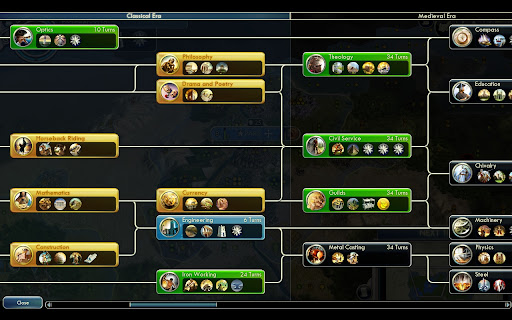
\includegraphics[scale=0.8]{resources/technology.jpg}}
\end{figure}

\subsection*{{\titr کارگرها و ستلرها}}
\addcontentsline{toc}{subsection}{{\fehrestContent کارگرها و ستلر ها}}

وقتی که یک کارگر فعال در موقعیتی است که می تواند فعالیتی انجام دهد، پنلی برای کار او نمایش داده شود. این پنل نشان می دهد که کارگر توانایی انجام چه کارهایی را دارد(به داک بازی مراجعه کنید). با کلیک بر روی آن کار، کارگر مشغول انجام آن کار می شود. کار کارگر زمان می برد و با نگه داشتن موس بر روی آن کار، باید مقدار زمانی که طول می کشد که آن کار به اتمام برسد نشان داده شود. برای این بخش، می توانید از یک progress bar استفاده کنید.
برای ستلر‌ها هم باید قابلیت احداث شهر وجود داشته باشد که همانند کارگر باید یک از طریق یک پنل در دسترس باشد.


\subsection*{{\titr دیپلماسی}}
\addcontentsline{toc}{subsection}{{\fehrestContent دیپلماسی}}

در فاز دوم پروژه شما باید قابلیت ارتباط با بقیه‌ی تمدن ها را طراحی کنید در این قسمت هر بازیکن باید بتواند با بقیه بازیکنان صحبت(discuss) و یا معامله(trade) کند. برای این قسمت باید پنلی وجود داشته باشد که بتوان تمام بازیکنان شناخته شده در بازی را مشاهده کرد و  امکان صحبت و معامله کردن با آن‌ها وجود داشته باشد. برای قسمت discuss پنلی باید وجود داشته باشد که بتوان با دیگر بازیکنان چت کرد(پیاده‌سازی کامل این قسمت برای فاز سوم است ولی شما باید در طراحی خود جایی برای این قابلیت در نظر بگیرید). برای قسمت trade باید پنلی وجود داشته باشد که شما بتوانید به بقیه بازیکنان پیشنهاد معامله بدهید. برای معامله شما می‌توانید مقداری گلد به ازای دریافت منابع دیگر(مانند اسب، زغال، …) بدهید یا بگیرید و سپس درخواست معامله باید برای بازیکن دیگر فرستاده شود(در این فاز کافی است در همان صفحه به بازیکن دیگر پیام معامله داده شود). همچنین در اتمام بازی، بازیکن برنده و اطلاعات امتیاز هر بازیکن نمایش داده شود.

\begin{figure}[H]
    \centerline{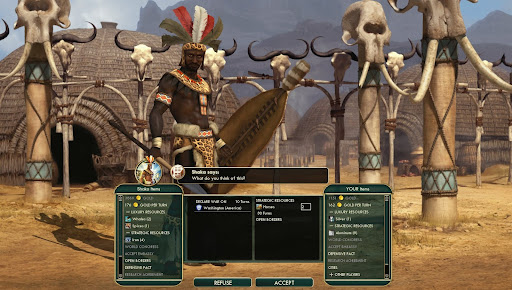
\includegraphics[scale=0.8]{resources/diplomacy.jpg}}
\end{figure}

\subsection*{\titr کد تقلب}
\addcontentsline{toc}{subsection}{{\fehrestContent کد تقلب}}
همانطور که به یاد دارید، در فاز 1 قابلیت کد تقلب برای انجام برخی از اعمال بازی وجود داشت. در این فاز شما باید یک محیط گرافیکی در بازی پیاده‌سازی کنید تا کاربر بتواند کدهای تقلب خود را وارد کند و آن‌ها را اعمال کند.
\\
\textbf{امتیازی:} همانطور که در منوی بازی نیز داشتید، شما میتونید در محیط بازی با زدن یک shortcut یک صفحه گرافیکی را بالا بیاورید و در آن کد تقلب خود را وارد و اعمال کنید. (مثلا با زدن دکمه‌های C+Shift+Ctrl یک صفحه سیاه مانند line command بالا بیاید و شما در آن کدهای تقلب خودرا وارد و اعمال کنید.)



\section*{{\titr نکات مهم}}
\addcontentsline{toc}{section}{{\fehrestContent نکات مهم}}

به‌طور کلی شما در فاز دوم، باید برای هر آنچه که در داک توضیحات بازی آمده است یک گرافیک مناسب پیاده‌سازی کنید.(حتی مواردی که در داک توضیحات بازی هستند اما در داک فاز دوم به آن‌ها پرداخته نشده است.)
\\
در صورتی که قسمت‌هایی از فاز 1 را تا هنگام تحویل آن فاز پیاده‌سازی نکرده بودید، میتوانید در این فاز پیاده‌سازی کرده، و 50 درصد نمره آن‌را برای فاز 1 دریافت کنید. (به طور مثال اگر قابلیت login را در فاز 1 پیاده‌سازی نکرده بودید اما در این فاز پیاده‌سازی کردید، در این فاز نمره کامل آن‌را دریافت می‌کنید و همچنین 50 درصد نمره آن در فاز 1 نیز برایتان ثبت خواهد شد.)\\
برای راحتی کار شما، همه مواردی که در هر چک پوینت باید پیاده سازی کنید آمده است. لطفا به زمان تحویل هر چک پوینت نیز دقت کنید.
\end{document}







